\subsection*{\lr{2.7.1} اثبات درستی}
  
  \begin{theorem}
  اگر جدول (tableau) \(\mathscr{T}\) برای فرمول \(A\) بسته شود، آنگاه \(A\) نارضایت‌پذیر \lr{unsatisfiable} است.
  \end{theorem}
  
  ما قضیه‌ای کلی‌تر را اثبات می‌کنیم:
  
  \begin{theorem}
  اگر زیر‌درخت \(\mathscr{T}_n\)، که در گرهٔ \(n\) از \(\mathscr{T}\) ریشه دارد، بسته باشد، آنگاه مجموعهٔ فرمول‌های \(U(n)\) که برچسب گرهٔ \(n\) است، نارضایت‌پذیر است.
  \end{theorem}
  
  درستیِ جدول (soundness) حالت خاصی از این قضیه است هنگامی که \(n\) همان گرهٔ ریشه باشد.
  
  برای سادگی اثبات، فرض می‌کنیم که فقط دو شکل از فرمول‌های \(\alpha\) و \(\beta\) داریم:
  \[
  \alpha\colon A_1 \land A_2,
  \qquad
  \beta\colon B_1 \lor B_2.
  \]
  
  \begin{proof}
  با استقرا بر ارتفاع \(h_n\) گرهٔ \(n\) در زیر‌درخت \(\mathscr{T}_n\).
  
  \textbf{قضیهٔ پایه} (\(h_n = 0\)).  
  اگر \(h_n=0\)، آنگاه \(n\) یک برگه (leaf) است و چون \(\mathscr{T}_n\) بسته است، در برچسب \(U(n)\) حتماً یک جفت متضاد از لیترال‌ها وجود دارد. بنابراین \(U(n)\) نارضایت‌پذیر است.
  
  \textbf{فرض استقرا}.  
  فرض کنید برای هر گرهٔ \(m\) با ارتفاع کمتر از \(h_n\) داریم:
  \[
  \forall m,\;h_m < h_n,\;\bigl[\mathscr{T}_m\ \text{بسته}\bigr]\;\Longrightarrow\;U(m)\ \text{نارضایت‌پذیر}.
  \]
  
  \textbf{گام استقرایی}.  
  حال گرهٔ \(n\) را در نظر بگیرید که \(h_n>0\). از آنجا که \(\mathscr{T}_n\) بسته است، حتماً روی \(n\) یکی از دو قاعدهٔ \(\alpha\) یا \(\beta\) اعمال شده است:
  \begin{center}
    \begin{latin}
      \resizebox{0.35\textwidth}{!}{
      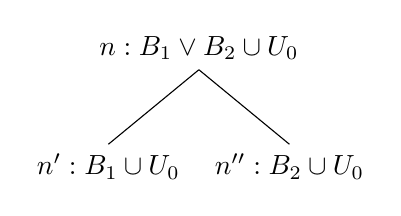
\begin{tikzpicture}[
        level distance=1.5cm,
        sibling distance=1.5cm,
        level 1/.style={sibling distance=2.3cm},
        edge from parent path={(\tikzparentnode.south) -- (\tikzchildnode.north)}
      ]
      \node {$n: {B_1 \lor B_2} \cup U_0$}
        child { 
          node {$n': {B_1} \cup U_0$}
        }
        child { 
          node {$n'': {B_2} \cup U_0$}
        };
      \end{tikzpicture}
      }  
    \hfill
    \resizebox{0.35\textwidth}{!}{
      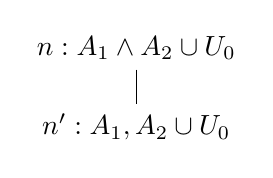
\begin{tikzpicture}[
        level distance=1cm,
        sibling distance=2.5cm,
        level 1/.style={sibling distance=2.5cm},
        level 2/.style={sibling distance=2.7cm},
        edge from parent path={(\tikzparentnode.south) -- (\tikzchildnode.north)}
      ]
      \node {$n: {A_1 \land A_2} \cup U_0$}
        child { node {$n': {A_1, A_2} \cup U_0$} };
      \end{tikzpicture}
      }
    \end{latin}
  \end{center}
  \begin{enumerate}[1)]
    \item \(\alpha\)\;  
      اگر قاعدهٔ \(\alpha\) (برای \(A_1\land A_2\)) روی \(n\) اعمال شده باشد، آنگاه
      \[
        U(n)=\{\,A_1\land A_2\}\cup U_0,
        \quad
        U(n')=\{\,A_1,\,A_2\}\cup U_0,
      \]
      و \(\mathscr{T}_{n'}\) نیز بسته است. از آنجا که ارتفاع \(n'\) برابر \(h_n-1\) است، به‌موجب فرض استقرا \(U(n')\) نارضایت‌پذیر است.  
      برای اثبات نارضایت‌پذیری \(U(n)\)، هر تفسیر دلخواه \(\mathscr{I}\) را در نظر بگیرید:
      \begin{itemize}
        \item اگر برای بعضی \(A_0\in U_0\)، \(v_{\mathscr{I}}(A_0)=F\)، چون \(U_0\subset U(n)\)، نتیجه می‌شود \(U(n)\) نارضایت‌پذیر است.
        \item در غیر این صورت \(v_{\mathscr{I}}(A_0)=T\) برای همهٔ \(A_0\in U_0\). چون \(U(n')\) نارضایت‌پذیر است، باید \(v_{\mathscr{I}}(A_1)=F\) یا \(v_{\mathscr{I}}(A_2)=F\).  
          اگر \(v_{\mathscr{I}}(A_1)=F\)، آنگاه
          \[
            v_{\mathscr{I}}(A_1\land A_2)=F,
          \]
          و چون \(A_1\land A_2\in U(n)\)، \(U(n)\) نارضایت‌پذیر است. (استدلال مشابه برای \(v_{\mathscr{I}}(A_2)=F\).)
      \end{itemize}
  
    \item \(\beta\)\;  
      اگر قاعدهٔ \(\beta\) (برای \(B_1\lor B_2\)) روی \(n\) اعمال شده باشد، آنگاه
      \[
        U(n)=\{\,B_1\lor B_2\}\cup U_0,\quad
        U(n')=\{\,B_1\}\cup U_0,\quad
        U(n'')=\{\,B_2\}\cup U_0,
      \]
      که هر دو \(\mathscr{T}_{n'}\) و \(\mathscr{T}_{n''}\) بسته‌اند و ارتفاع‌شان کمتر از \(h_n\) است. بنابراین \(U(n')\) و \(U(n'')\) نارضایت‌پذیرند.  
      برای هر تفسیر \(\mathscr{I}\):
      \begin{itemize}
        \item اگر برای بعضی \(B_0\in U_0\)، \(v_{\mathscr{I}}(B_0)=F\)، چون \(U_0\subset U(n)\)، آنگاه \(U(n)\) نارضایت‌پذیر است.
        \item وگرنه \(v_{\mathscr{I}}(B_0)=T\) برای همهٔ \(B_0\in U_0\).  
          از نارضایت‌پذیری \(U(n')\) و \(U(n'')\) داریم \(v_{\mathscr{I}}(B_1)=F\) و \(v_{\mathscr{I}}(B_2)=F\).  
          بنابراین
          \[
            v_{\mathscr{I}}(B_1\lor B_2)=F,
          \]
          و چون \(B_1\lor B_2\in U(n)\)، \(U(n)\) نارضایت‌پذیر است.
      \end{itemize}
  \end{enumerate}
  
  در هر دو حالت، نشان دادیم که اگر زیر‌درختهای فرزندان \(n\) بسته باشند، آنگاه \(U(n)\) نیز نارضایت‌پذیر است. این کامل‌کنندهٔ گام استقرایی است.
  
  بنابراین، به‌موجب اصل استقرا، برای هر گره \(n\)، اگر زیر‌درخت \(\mathscr{T}_n\) بسته باشد، آنگاه \(U(n)\) نارضایت‌پذیر است. حالت ویژه برای گرهٔ ریشه (\(n=\text{root}\)) اثبات می‌کند که اگر کل جدول \(\mathscr{T}\) بسته شود، آنگاه فرمول اولیه \(A\) نارضایت‌پذیر است.
  \end{proof}